\chapter{Literature Review \& Work Done}

%\todo{Analyse, synthesize critically evaluate}

\section{Alcohol Harm Paradox}

The \ac{AHP} has emerged from a collection of literature, where the association of alcohol harms with \ac{SES} was first formalised by Smith et al.~in 2014 \cite{ahpOrigin}. Health inequalities have been apparent in almost all civilisations to date, and have even been shown to emerge as a result of being low status in the animal kingdom \cite{primateSocialDeterminants, Krieger1997}. The question becomes why in a modern society with relatively widespread access to healthcare and health information is \ac{SES} still a key determining factor in someone's health? And what are the other risk factors that determine the  difference in health outcomes in the context of alcohol consumption?

The Global Status Report on Alcohol 2018 by the \ac{WHO} points numerous times to \ac{SES} being a key determining factor for  differential outcomes in alcohol harms. On a global level, with Europe and North America having the highest alcohol consumption rates, low and lower-middle-income countries experience the highest levels of harm related to alcohol \cite{WHOGlobalStatusReportFull}. Even within the bounds of the global regions declared by the \ac{WHO}, the \ac{AHP} was still apparent \cite{WHOGlobalStatusReportFull}. It is, therefore, appropriate to state that the \ac{AHP} is a phenomenon that occurs across scales. 

Boyd et al.~conducted a systematic literature review which looked for explanations of the \ac{AHP} \cite{Boyd2022}. The fact this was conducted in 2022 implies that the \ac{AHP} is still not well understood. Boyd notes a significant gap in the literature surrounding the \ac{AHP} is the lack of research surrounding social and economic causes. A number of reports from the UK demonstrate and investigate the \ac{AHP} \cite{scotlandAlcohol2022, ahpInterventions, ahp2016, ahpWhatNext}. 

Research by Bellis et al.~acknowledges the \ac{AHP} and reasons that individual-based actions such as smoking and diet choices alongside less access to healthcare resources may lead to the \ac{AHP} \cite{ahp2016}. Research performed by Baldwin et al.~suggested five hypotheses for the existence of the \ac{AHP} \cite{ahpInterventions}. Baldwin then tested three of these including under-reporting of alcohol use, drinking patterns between \ac{SES} groups and compounding effects of other health determinant factors such as diet and physical activity. Baldwin did not test differences in access to health services between different \ac{SES} groups or whether the \ac{AHP} could be explained by individuals with problematic alcohol habits moving into lower \ac{SES} positions as a result of their consumption. Baldwin finally points towards a lack of published evidence that looks at the underlying mechanisms behind the \ac{AHP}. 
\pagebreak

A theme in the literature is the lack of access to healthcare in low \ac{SES} communities as a leading contributing factor behind the \ac{AHP}. This can be linked to the inverse care law - first noted in 1971, and a well known problem in public health \cite{inverseCareLaw}. The literature to date attributes the \ac{AHP} to a variety of causal mechanisms alongside differential access to healthcare. It is clear that there are multiple factors contributing to the \ac{AHP}. Although certain individual behaviours are thought to contribute towards the \ac{AHP} the literature in general misses the broader social and economic context. This is peculiar considering the \ac{AHP} is inherently a social problem.

There is literature proposing complex systems approaches could be used to investigate health disparities, which would address the lack of social and economic context in the \ac{AHP} literature \cite{csHealthDisparities, Boyd2021}. Particularly, Boyd et al.~suggest four health inequality theories could be used to investigate the \ac{AHP}, one of which is \ac{FCT}, which is what this dissertation will focus on modelling\cite{Boyd2021}. 

%\todo{discuss possible interventions with jens paper and the interventions paper}

%\todo{Lifestyle risk factors have not been accounted for}

%\todo{What are the criticisms if any? - lifestyle and other risk factors to do with low SES}

%\todo{gaps in literature? could lead onto fct?}


\section{Fundamental Cause Theory}

First noted by Link et al.~\ac{FCT} proposes that socioeconomic conditions are the underlying causes of disease, under the precipice that negative health outcomes cannot be resolved solely by addressing the direct mechanisms associated with the disease itself \cite{FCTorigin}. It recognises that, for example, a person with an \ac{AUD} will struggle to resolve the issue through individual action if the social and economic resources available to them are low. By contrast someone with  access to healthcare, money, knowledge, a supportive community and holds a position of high prestige in society is more likely to overcome adverse effects of \ac{AUD}. 

There are two ways to test whether \ac{FCT} can successfully explain a phenomenon \cite{fctRetro}. First is the \say{preventability shifts approach}, which looks at exposure to different diseases over time as well as the capacity to cure said diseases. When the capacity to cure a disease increases, if low \ac{SES} individuals are seen to have a higher mortality rate then \ac{FCT} can be used to explain the phenomenon.
The second is the \say{Manipulated preventability approach} where given a sample of a population when interventions are performed on a random set of individuals but require resources to benefit from the interventions, if differential health outcomes are observed based on access to resources then \ac{FCT} can be used to explain the phenomenon.

%Link notes that \say{fundamental causes are linked to multiple disease outcomes through multiple risk-factor mechanisms}, meaning that 

\ac{FCT} has seen success in explaining neighbourhood disadvantage and differential outcomes from both mental and physical health issues \cite{fctNeighbourhoods, fctStressors, fctLungCancerUS}. For hard-to-cure diseases \ac{FCT} is less effective in predicting health outcomes \cite{fctLungCancerUS}. This suggests that \ac{FCT} cannot explain all health outcomes in society, but can be used to attribute differential health outcomes for individuals with different \ac{SES} for curable diseases. Common diseases of the liver are largely curable or preventable, and liver damage is often linked to alcohol consumption. Common advice given to either prevent or aid the recovery of liver diseases is to abstain from or reduce alcohol consumption \cite{liverDiseaseList}. 

Boyd et al.~\cite{Boyd2021} note that \ac{FCT} is not apparent in \ac{AHP} literature and argues that individual-based methods for understanding the \ac{AHP} are limited as they fail to account for the socio-economic context in which people live. This was the original motivation behind the research done by Link \cite{FCTorigin}. \ac{FCT} seems to be useful social theory to help unravel the \ac{AHP} due to the strong link between \ac{AHP} and \ac{SES}.

%\todo{What are the criticisms if any?} 

%\todo{Critical Evaluation of FCT explaining AHP}

%\todo{when mentioning SES mention IMD quintiles and their purpose}


\section{Agent-based Models in Public Health}

\todo{Agent Rules}
\todo{MBSSM (8 pages)}
\todo{Describe Agents}
\todo{Describe Environment}
\todo{describe rules}
\todo{describe other methods with which to attack this problem ie what other ways apart from abm}




\ac{ABM}s give researchers and policymakers the capacity to model how \textit{local interactions} lead to the emergence of complex, large-scale behaviour \cite{abmEpstein, abmGeneral}. \ac{ABM}s have had success in explaining social phenomena such as segregation \cite{schelling}.  One of the more recent applications of agent-based modelling in public health was during the COVID-19 pandemic, where \ac{ABM}s were used to evaluate and justify stay-at-home orders \cite{covidABM}. 

A scoping literature review was conducted by McGill et al.~which looked for literature which used complex systems approaches in exploring alcohol related harms, some of which included \ac{ABM}s \cite{scopingReview}. Some \ac{ABM}s focus on alcohol consumption among young and college-aged people \cite{collegeABMCLD, abmCollegeConsumption, abmCollegePolicyandMechanisms, abmYoungAus, abmNetLogo}, whilst others investigate more general populations \cite{abmBinge, abmAlcoholTaxation, abmDutchAdults, abmDrinkingBehaviour, abmEcologicalNiche, abmTradingHours, abmPublicTransport}. 
Certain \ac{ABM}s focus on alcohol consumption during events where alcohol is consumed, such as nights out or parties with the intention of finding ways to reduce alcohol related violence \cite{abmVenueLock, abmPublicTransport, abmAlcoholCrime, abmSimARC, abmDrinkingBehaviour, abmEcologicalNiche, abmTradingHours, abmRiskBehaviourDev}. There are also some \ac{ABM}s prioritising intervention strategies \cite{collegeABMCLD, abmVenueLock, abmPublicTransport, abmNetLogo, abmPolicyInterventions, abmCollegePolicyandMechanisms, abmAlcoholTaxation, abmDrinkingBehaviour} and some prioritising understanding behavioural mechanisms \cite{collegeABMCLD, abmRiskBehaviourDev, abmYoungAus, abmCollegeConsumption, abmCollegePolicyandMechanisms, abmAlcoholCrime, abmBinge, abmSimARC, abmDutchAdults, abmDrinkingBehaviour, abmEcologicalNiche}. There is notable overlap between \ac{ABM}s which look at behaviour and intervention strategies, as often understanding of behaviour is needed before the appropriate strategies can be employed. The models which are based on real-world data are initialised based on data sets from the US, UK, The Netherlands and Australia, hence there is a bias towards analysing populations from more advanced economies.

A common theme in the literature  is to help shape types of interventions to curb the negative effects of alcohol by attempting to outline the mechanisms related to problematic alcohol consumption. Many of these models focus on the direct harms associated with events related to alcohol consumption such as alcohol related violence, trips and falls and vehicle-related accidents. No \ac{ABM}s mentioned in McGill's review focus on \ac{SES} or the \ac{AHP}. This may suggest that \ac{ABM} as a technique may not be suitable for investigating the \ac{AHP}, but other computational complex systems approaches, such as dynamic systems modelling, fail to capture the complexity involved where there are multiple interacting agents such as in a population. 

A framework developed by Vu et al.~presents a method with which \ac{ABM}s can be built to analyse social theories by modelling the underlying theory mechanisms \cite{MBSSM}. Vu refers to this framework as \ac{MBSSM}, which allows developers to create agent based models to model macro-micro, micro-micro, micro-macro interactions. \ac{MBSSM} has since been used to develop the \ac{MUP} policy in Scotland \cite{mbssmCommentary, scotlandMUP}. Boyd et al.~ state that with the advent of \ac{MBSSM} twinned with the interest of policymakers to use \ac{ABM}-based tools, it is an appropriate time to investigate the \ac{AHP} through \ac{ABM}s \cite{Boyd2022, sipherIntro}

Summarising, there is a clear gap in the \ac{AHP} literature, which has failed in finding the underlying causes of the \ac{AHP} due to the reliance on individual-based interventions. \ac{FCT} presents a new theory to investigate the \ac{AHP},  proposing that \ac{SES} and the difficulties and lack of resources that accompany being low \ac{SES} lead to the differential outcomes in alcohol harms described by the \ac{AHP}. \ac{ABM}s have seen success in public health modelling and in finding intervention strategies for dealing with alcohol related harms and \ac{ABM} seems like an appropriate technique to investigate whether \ac{AHP} can be explained through \ac{FCT}, especially since the development of the \ac{MBSSM} framework. 

%\todo{bridging between theory and own work. Jen developed abm, used mbssm, look at reproducing the conceptual model, }

%\todo{mbssm will be worth more pages in the dissertation (approx 2) }





%Recently alcohol policy in Scotland... minimum unit pricing... derived from ABM SAPM... 

%The purpose of this dissertation is to develop and build an \ac{ABM} to see whether it is feasible to firstly see if FCT is a reasonable theory to understand AHP, but also to lay the groundwork for further development of the model to be enhanced. 

\section{Work Done}




\subsection{ODD}

The \ac{ODD} protocol is a standard protocol used to describe how a particular \ac{ABM} works \cite{oddOrigin}. Boyd produced an \ac{ABM} to analyse whether \ac{FCT} could describe the \ac{AHP} \cite{BoydphD}. This dissertation takes inspiration from Boyd's work and seeks to replicate and extend the model, and explore the fundamental behaviours. The full \ac{ODD} will be given in the final dissertation; the initial overview and design is given below.

\subsubsection{Overview}
The model proposed takes mechanisms present in \ac{FCT} and looks to explore the model output space with the intention of model exploration. The agents in the model live in an environment determined by a \ac{DQ}. The agents are exposed to alcohol harm through drinking at a rate linked to their individual propensity to drink. The event generator periodically broadcasts events to a random number of agents events that help agents avoid alcohol harms. The level to which agents can decode the information is in part determined by \ac{FCT}-related parameters. Events are stored by the agent and each tick the agent will attempt to solve an event they've not yet solved. Agents have the capacity to share a successful adaptation to the event information with an agent within their social network once per tick. 

\subsection{Software Design}
\ac{UML} is an approach to software design which presents many benefits in the development of \ac{ABM}s \cite{UMLABM}. Class diagrams, which are used to describe the behaviour of and relationship between entities in a model, are said to be among the most important model to design in the development of \ac{ABM}s \cite{UMLABM}. Figure \ref{fig:fctUML} shows the current \ac{UML} diagram that follows the \ac{MBSSM} framework but re-contextualises the example model given in the paper to account for only \ac{FCT} in terms of social theories. There has been an extension to the \ac{MBSSM} example with the inclusion of a social network and environment classes, and the exclusion of mediator classes. Further details will be discussed in the final dissertation.

\begin{figure}[h]
\centering
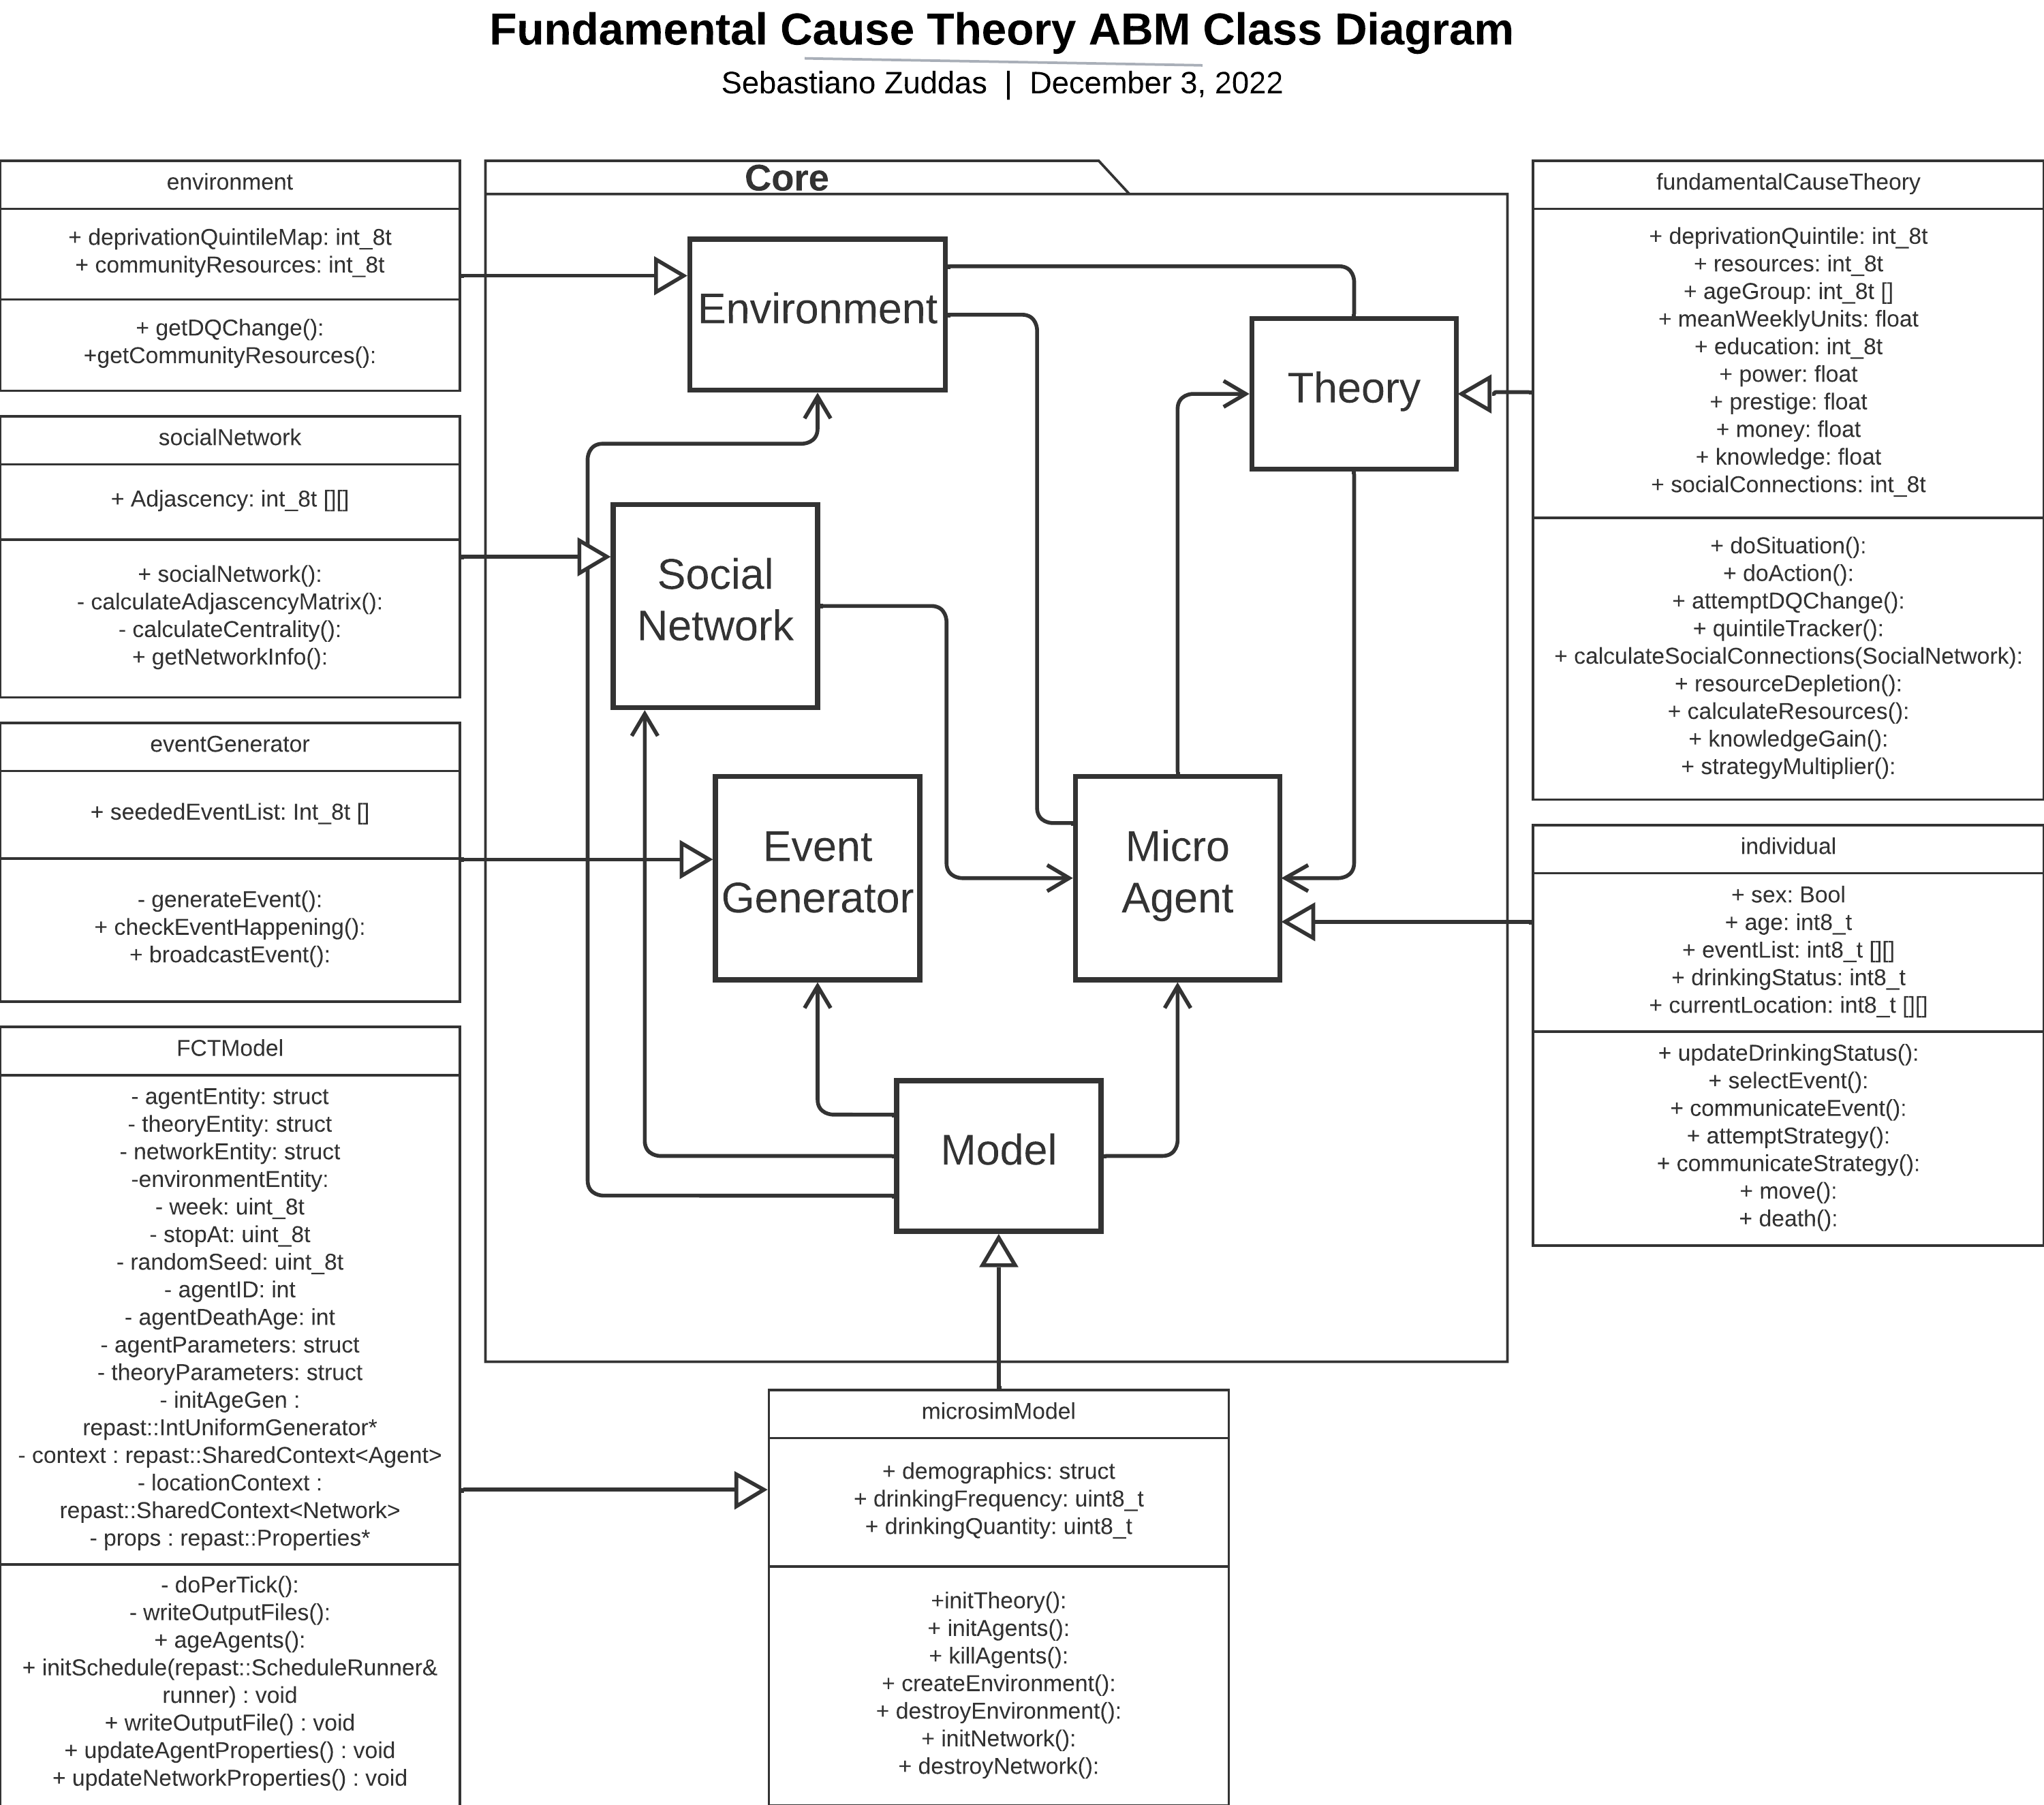
\includegraphics[width=\linewidth]{figures/Class Diagram FYP December.png}
\caption{A class diagram of the proposed ABM}
\label{fig:fctUML}
\end{figure}


% \subsection{Relevant Equations on Mechanisms of Action}
% \begin{figure}[h]
% \centering
% 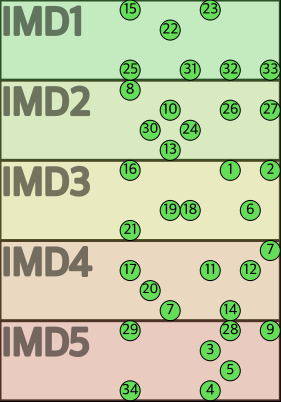
\includegraphics[scale=0.5]{USFD_Academic-_Report_LaTeX-Template/figures/ABM Diagram Single Year.png}
% \caption{An example graph}
% \label{fig:x cubed graph}
% \end{figure}


\subsection{Experiment Conceptualisation}

Table \ref{tab:experiments} shows a number of experiment concepts that has been reduced in the interest of keeping within the report requirements. The most important experiment that will be conducted is parameter space exploration through \ac{LHS}, a technique used to generate a set of parameters for this purpose. This is intended to demonstrate the general behaviour of the model and give insight into expected and unexpected behaviours. Other experiments, such as those related to \ac{FCT} and \ac{AHP} give credibility to the model. Finally, an interesting experiment would be to look at which \ac{FCT}-related parameters lead to the gratest harm, giving scope for further research and potential development for the model.  

\begin{table}[H]
\centering
\begin{tabular}{||p{0.3\textwidth}|p{0.3\textwidth}|p{0.3\textwidth}||}
 \hline
    Experiment & Method & Expected Impact \\[0.5ex] 
 \hline\hline
  Exploration of the parameter space. & Using \ac{LHS}. & Demonstrate general model behaviour. \\ 
  \hline
  Can \ac{FCT} be shown?  & Preventability shifts,  manipulated preventability. & Validation of \ac{FCT} working in the model. \\
  
  \hline
  Can \ac{AHP} be shown? & Changing the extremities of available community and individual resources & Further evidence that \ac{AHP} can be explained through \ac{FCT}. \\
  \hline
  
  Which \ac{FCT} parameters relate most to alcohol harm? & Test extremities of each \ac{FCT} parameter. & A certain combination of parameters will lead to the most harm for all individuals. \\ [1ex] 
 \hline
\end{tabular}
\caption{Table showing initial experiment concepts.}
\label{tab:experiments}
\end{table}

